\documentclass{problem-set}
\usepackage{graphicx}
\graphicspath{ {./images/} }

\title{Problem Set}
\subheader{SLSS Computer Science Club}
\date{October 5, 2018}
\author{David Tsukernik}

\begin{document}
\maketitle

\section{Best Fish (Difficulty: Easy)}
Two friends, Casper and Natalie went fishing. They caught a lot of fish. Casper pointed out that he had the longest fish, but Natalie said she had the heaviest fish. They agreed that they would determine the best fish as being the one whose product of the weight and length was the largest.

Your job is to determine who caught the best fish.

\inputformat
The input begins with an integer $C (\leq10000)$ which represents the total number of fish that Casper caught. Then each of the $C$ records follows on its own line. Each record consists of two positive integers each less than 10000: the weight followed by the length of that particular fish. After these records, there is a number $N (\leq10000)$ which represents the total number of fish that Natalie caught.
On the next $N$ lines, there is one record per line, as outlined above.
\outputformat
The output will be \textbf{Casper} if he has caught the best fish, or  \textbf{Natalie} if she has caught the best fish, or  \textbf{Tie} if they caught equally good fish.

\pushnewpage

\addsample
{
3\\
10 3\\
3 11\\
4 4\\
4\\
10 2\\
29 1\\
16 2\\
6 6
}
{
Natalie
}

\section{The Candy Mountain (Difficulty: Medium)}
In order to ensure peace and prosperity for future generations, the United Nations is creating the world's largest candy. The ingredients must be taken in railway cars from the top of a mountain and poured into Lake Geneva. The railway system goes steeply from the mountaintop down to the lake, with a T-shaped branch in the middle as shown below.

\begin{figure}[h]
    \centering
    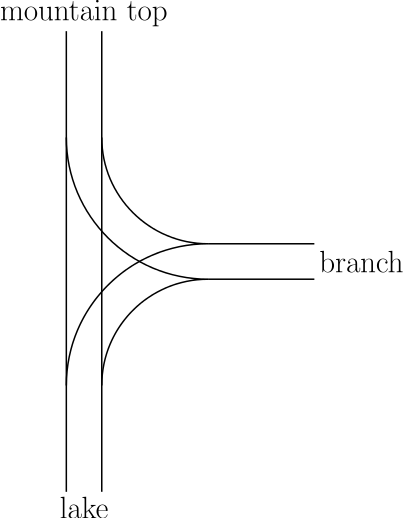
\includegraphics[scale=0.5]{the-candy-mountain-1}
\end{figure}

\pushnewpage

Right now, each of the $N$ ingredients is in its own railway car. Each railway car is assigned a positive integer from 1 to $N$. The ingredients must be poured into the lake in the order 1,2,3,…,$N$ but the railway cars are lined up in some random order. The difficulty is that, because of the especially heavy gravity today, you can only move cars downhill to the lake, or sideways on the branch line. Is it still possible to pour the ingredients into the lake in the order 1,2,3,…,$N$?

For example, if the cars were in the order 2, 3, 1, 4, we can slide these into the lake in order as described below:

\begin{figure}[h]
    \centering
    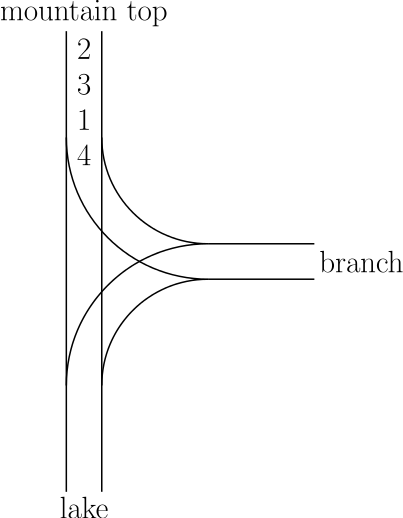
\includegraphics[scale=0.5]{the-candy-mountain-2}
\end{figure}

\begin{itemize}
    \item Slide car 4 out to the branch
    \item Slide car 1 into the lake
    \item Slide car 3 out to the branch
    \item Slide car 2 into the lake
    \item Slide car 3 from the branch into the lake
    \item Slide car 4 from the branch into the lake
\end{itemize}

\inputformat
The first line will contain the number $T (1 \leq T \leq 10)$ which is the number of different tests that will be run. Each test has the form of an integer $N (1 \leq N \leq 100000)$ on the first line of the test, followed by a list of the $N$ cars listed from top to bottom. The cars will always use the numbers from 1 to $N$ in some order.

\pushnewpage

\outputformat
For each test, output one line which will contain either  \textbf{Y} (for "yum") if the recipe can be completed, and  \textbf{N} otherwise.

\addsample
{
2\\
4\\
2\\
3\\
1\\
4\\
4\\
4\\
1\\
3\\
2
}
{
Y\\
N
}

\section{Mess (Difficulty: Hard)}
In the nearby kindergarten they recently made up an attractive game of strength and agility that kids love.

The surface for the game is a large flat area divided into $N\times N$ squares.

The children lay large spongy cubes onto the surface. The sides of the cubes are the same length as the sides of the squares. When a cube is put on the surface, its sides are aligned with some square. A cube may be put on another cube too.

Kids enjoy building forts and hiding them, but they always leave behind a huge mess. Because of this, prior to closing the kindergarten, the teachers rearrange all the cubes so that they occupy a rectangle on the surface, with exactly one cube on every square in the rectangle.

In one moving, a cube is taken off the top of a square to the top of any other square.

Write a program that, given the state of the surface, calculates the smallest number of moves needed to arrange all cubes into a rectangle.

\pushnewpage

\inputformat
The first line contains the integers $N$ and $M (1\leq N\leq 100,1\leq M\leq N^2)$, the dimensions of the surface and the number of cubes currently on the surface.

Each of the following M lines contains two integers $R$ and $C (1\leq R,C\leq N)$, the coordinates of the square that contains the cube.

\outputformat
Output the smallest number of moves. A solution will always exist.

\addsampleExplanation
{
3 2\\
1 1\\
1 1
}
{
1
}
{
It suffices to move one of the cubes from (1, 1) to (1, 2) or (2, 1).
}

\pushnewpage

\addsampleExplanation
{
5 8\\
2 2\\
3 2\\
4 2\\
2 4\\
3 4\\
4 4\\
2 3\\
2 3
}
{
3
}
{
A cube is moved from (2, 3) to (3, 3), from (4, 2) to (2, 5) and from (4, 4) to (3, 5).
}

\end{document}